% =============================================================================
% RESUMEN EJECUTIVO GERENCIAL - PROYECTO P2611
% Análisis Fondo Tanque Glucosa - Ingredion S.A.
% DML Ingenieros Consultores S.A.S.
% =============================================================================
\documentclass[12pt,a4paper]{elsarticle}

% ===================== DATOS ESPECÍFICOS DEL DOCUMENTO =====================
% ===================== DATOS DEL PROYECTO =====================
% Resumen Ejecutivo Gerencial - P2611-PR-INF-003

% 1. Información General del Proyecto
\newcommand{\projecttitle}{Revision Térmica y Estructural del Fondo del Tanque de Almacenamiento de Glucosa}
\newcommand{\doctitleshort}{RESUMEN EJECUTIVO GERENCIAL}
\newcommand{\documentcode}{P2611-PR-INF-003}
\newcommand{\documenttype}{RESUMEN EJECUTIVO GERENCIAL}
\newcommand{\targetcompany}{P2611}

% 2. Información de Documento y Emisión
\newcommand{\docRevision}{0}
\newcommand{\docFecha}{\today}
\newcommand{\docFechaLarga}{ABRIL 14 2026}

% 3. Integrantes y Control de Firmas
\newcommand{\firmaElaboro}{J. Arboleda}
\newcommand{\firmaReviso}{David Gómez}
\newcommand{\firmaAprobo}{H. Rosero}

% 4. Fechas de Firmas y Revisiones
\newcommand{\fechaElaboro}{ABRIL 14 2026}
\newcommand{\fechaReviso}{ABRIL 14 2026}
\newcommand{\fechaAprobo}{ABRIL 14 2026}

% 5. Datos de Historial de Revisiones (Portada / Firmas)
\newcommand{\fechaRevCero}{ABRIL 14 2026}
\newcommand{\descRevCero}{Emisión inicial del Resumen Ejecutivo Gerencial}
\newcommand{\fechaRevUno}{--}
\newcommand{\descRevUno}{Revisión cliente}
\newcommand{\fechaRevDos}{--}
\newcommand{\descRevDos}{Emisión final}
\newcommand{\fechaRevTres}{--}
\newcommand{\descRevTres}{--}
\newcommand{\fechaRevCuatro}{--}
\newcommand{\descRevCuatro}{--}


% ===================== IMPORTAR CONFIGURACIÓN MODULAR =====================
% ===================== CONFIGURACIÓN DE PÁGINA MEJORADA =====================
\pdfminorversion=7
\usepackage[top=4.5cm, bottom=2.5cm, left=2.0cm, right=2.0cm,
headheight=4cm, headsep=0.5cm]{geometry}

% ===================== TIPOGRAFÍA Y CODIFICACIÓN =====================
\usepackage[utf8]{inputenc}
\usepackage[T1]{fontenc}
\usepackage[spanish,es-tabla]{babel}
\usepackage{tgtermes}
\usepackage{microtype}
\usepackage{textcase}


% Forzar justificaci\'on expl\'icita en todo el documento (LaTeX justifica por defecto)
\tolerance=1000
\emergencystretch=3em
\hyphenpenalty=50
\exhyphenpenalty=50

% ===================== ELIMINAR SANGRÍAS =====================
\usepackage[parfill]{parskip}
\setlength{\parindent}{0pt}
\setlength{\parskip}{6pt}
\AtBeginDocument{\setlength{\parindent}{0pt}}
\AtBeginDocument{\setlength{\parskip}{6pt}}

% ===================== CONFIGURACIÓN DE TÍTULOS =====================
\usepackage{titlesec}
\titleformat{\section}{\bfseries\fontsize{12}{14}\selectfont}{\thesection}{1em}{}
\titleformat{\subsection}{\bfseries\fontsize{12}{14}\selectfont}{\thesubsection}{1em}{}
\titleformat{\subsubsection}{\bfseries\fontsize{12}{14}\selectfont}{\thesubsubsection}{1em}{}
\titleformat{\paragraph}{\bfseries\fontsize{11}{13}\selectfont}{\theparagraph}{1em}{}
\titlespacing*{\paragraph}{0pt}{2.5ex plus 0.5ex minus 0.2ex}{1ex plus 0.2ex}

% ===================== PAQUETES MATEMÁTICOS =====================
\usepackage{amsmath,amssymb,amsfonts,mathtools}
\usepackage{textgreek,gensymb,siunitx}

% ===================== QUÍMICA Y SÍMBOLOS =====================
\usepackage[version=4]{mhchem}
\usepackage{chemfig,textcomp}

% ===================== TABLAS Y FIGURAS =====================
\usepackage{booktabs,array,longtable,multirow}
\usepackage{graphicx,float,subcaption}
\usepackage{tabularx}

% ===================== SOPORTE PARA SVG =====================
\usepackage{svg}

% ===================== ENLACES E HIPERVÍNCULOS =====================
\usepackage[hidelinks,colorlinks=true,linkcolor=blue,citecolor=blue]{hyperref}
\usepackage{url}

% ===================== OTROS PAQUETES =====================
\usepackage{enumitem,xcolor,listings,algorithm,algpseudocode}
\usepackage{tocloft}
\usepackage{appendix}
\usepackage{eso-pic}
\usepackage{lastpage}

% ===================== PAQUETES ADICIONALES PARA TABLAS ESTÉTICAS =====================
\usepackage[table]{xcolor} % Colores en tablas (rowcolor, cellcolor)
\usepackage{colortbl}

% ===================== AUTO-NUMERACIÓN DE TABLAS =====================
\newcounter{itemcount}
\newcolumntype{N}{>{\stepcounter{itemcount}\theitemcount}c}

% ===================== CONFIGURACIÓN DEL ENCABEZADO =====================
\usepackage{fancyhdr}

% Desactivar marcas de secci\'on para evitar conflictos con acentos en
% los encabezados generados autom\'aticamente por elsarticle
\renewcommand{\sectionmark}[1]{}
\renewcommand{\subsectionmark}[1]{}
\renewcommand{\subsubsectionmark}[1]{}

% ===================== INFORMACIÓN DEL DOCUMENTO =====================
% Nota: El archivo de datos del proyecto se carga externamente en el
% documento maestro antes de importar este preamble.tex.

% Adaptaciones para el encabezado corporativo
\newcommand{\documentrevision}{REV \docRevision}
\newcommand{\documentdate}{\docFechaLarga}
\newcommand{\elaboratedby}{\MakeUppercase{\firmaElaboro}}
\newcommand{\reviewedby}{\MakeUppercase{\firmaReviso}}
\newcommand{\approvedby}{\MakeUppercase{\firmaAprobo}}

% ===================== CONFIGURACIÓN DE LISTINGS =====================
\lstset{
	basicstyle=\footnotesize\ttfamily,
	breaklines=true,
	frame=single,
	language=Python,
	showstringspaces=false
}

% ===================== ENCABEZADO NATIVO =====================
\newcommand{\empresaheader}{%
	\renewcommand{\arraystretch}{0.80} % Comprime la altura de las filas
	\noindent
	\begin{tabularx}{\textwidth}{@{}>{\centering\arraybackslash}p{2.5cm}>{\centering\arraybackslash}p{2.5cm}>{\centering\arraybackslash}X p{2cm} p{3cm}@{}}
		\toprule
		% Fila 1
		\multirow{5}{*}{
\includegraphics[width=2.3cm,height=2.5cm,keepaspectratio]{logos/logo1.png}} & 
		\multirow{5}{*}{
\includegraphics[width=2.3cm,height=2.5cm,keepaspectratio]{logos/logo2.png}} & 
		\multirow{2}{\linewidth}{\centering \scriptsize DISE\~NO DE INGENIER\'IA} & 
		\scriptsize \textbf{C\'DIGO:} & \scriptsize \documentcode \\ \cmidrule(l){4-5}
		
		% Fila 2
		& & & \scriptsize \textbf{REVISI\'ON:} & \scriptsize \documentrevision \\ \cmidrule(l){3-5}
		
		% Fila 3
		& & \multirow{2}{\linewidth}{\centering \scriptsize \documenttype} & 
		\scriptsize \textbf{FECHA:} & \scriptsize \documentdate \\ \cmidrule(l){4-5}
		
		% Fila 4
		& & & \scriptsize \textbf{ELABOR\'O:} & \scriptsize \elaboratedby \\ \cmidrule(l){3-5}
		
		% Fila 5
		& & \multirow{2}{\linewidth}{\centering \scriptsize \doctitleshort} &
		\scriptsize \textbf{REVIS\'O:} & \scriptsize \reviewedby \\ \cmidrule(l){1-2} \cmidrule(l){4-5}
		
		% Fila 6
		\textbf{\scriptsize PROYECTO:} & \scriptsize \targetcompany & & \scriptsize \textbf{APROB\'O:} & \scriptsize \approvedby \\ \bottomrule
	\end{tabularx}%
}

% ===================== ESTILO CORPORATIVO DEFINITIVO =====================
\fancypagestyle{corporativo}{%
	\fancyhf{} % Limpia todo
	\fancyhead[C]{\empresaheader} % Membrete centrado
	\fancyfoot[C]{%
		\fontsize{9}{11}\selectfont\color{gray}%
		 Cali - Colombia \\
		E-mail: [correo@empresa.com]}
	\fancyfoot[R]{%
		\fontsize{6}{8}\selectfont%
		CI-ESP-001\_R0 \\%
		P\'agina \thepage\ de \pageref{LastPage}}
	\renewcommand{\headrulewidth}{0pt} % Sin línea
	\renewcommand{\footrulewidth}{2pt} % Línea gruesa negra en pie
}

% Aplicar estilo globalmente
\pagestyle{corporativo}

% ===================== FORZAR ESTILO EN TODOS LOS CONTEXTOS =====================
\makeatletter
% Redefinir todos los estilos de página posibles para usar el nuestro
\let\ps@plain\ps@corporativo
\let\ps@empty\ps@corporativo
\let\ps@headings\ps@corporativo
\let\ps@myheadings\ps@corporativo

% CRÍTICO: Interceptar y redefinir el estilo del frontmatter de Elsevier
\let\ps@pprintTitle\ps@corporativo
\let\ps@pprintFirstpage\ps@corporativo
\makeatother


\journal{Revista de Ingeniería}

\begin{document}

% ===================== IMPORTAR SECCIONES MODULARES =====================
% ===================== HOJA DE FIRMAS =====================
\begin{titlepage}
	\thispagestyle{corporativo}

	\vspace*{1.5cm}

	% Título del informe
	\centering
	{\Large\bfseries \projecttitle}

	\vspace{4cm}

	% ==================== DATOS EDITABLES ====================
	% (La información ahora es dinámica y fluye desde config/datos_proyecto.tex)

	% Definir columnas personalizadas
	\newcolumntype{C}{>{\centering\arraybackslash}X}
	\newcolumntype{G}{>{\centering\arraybackslash}p{0.28\textwidth}}
	\newcolumntype{H}{>{\centering\arraybackslash}p{0.12\textwidth}}
	\newcolumntype{I}{>{\centering\arraybackslash}p{0.20\textwidth}}

	% Tabla 1: Control de Elaboración
	\centering
	\fontsize{10}{12}\selectfont
	\renewcommand{\arraystretch}{1.3}
	\setlength{\tabcolsep}{3pt}

	\begin{tabular}{|p{0.3\textwidth}|p{0.3\textwidth}|p{0.3\textwidth}|}
		\hline
		\rowcolor{green!15}
		\textbf{Elaborado por:} & \textbf{Revisado por:} & \textbf{Aprobado por:} \\
		\hline
		\centering\arraybackslash\rule{0pt}{1.5cm} \firmaElaboro & \centering\arraybackslash\rule{0pt}{1.5cm} \firmaReviso & \centering\arraybackslash\rule{0pt}{1.5cm} \firmaAprobo \\
		\hline
		\centering\arraybackslash Fecha: \fechaElaboro & \centering\arraybackslash Fecha: \fechaReviso & \centering\arraybackslash Fecha: \fechaAprobo \\
		\hline
	\end{tabular}

	\vspace{2.5cm}

	% Tabla 2: Control de Revisiones
	\centering
	\fontsize{10}{12}\selectfont
	\renewcommand{\arraystretch}{1.2}
	\setlength{\tabcolsep}{3pt}

	\begin{tabular}{|c|c|p{0.3\textwidth}|c|c|c|}
		\hline
		\rowcolor{green!15}
		\textbf{Versión} & \textbf{Autor} & \textbf{Descripción} & \textbf{Fecha elab.} & \textbf{Fecha rev.} & \textbf{Revisado por} \\
		\hline
		REV\docRevision & \firmaElaboro & \descRevCero & \fechaElaboro & \fechaReviso & \firmaReviso \\
		\hline
		REV1 & -- & \descRevUno & \fechaRevUno & -- & -- \\
		\hline
		REV2 & -- & \descRevDos & \fechaRevDos & -- & -- \\
		\hline
		REV3 & -- & \descRevTres & \fechaRevTres & -- & -- \\
		\hline
		REV4 & -- & \descRevCuatro & \fechaRevCuatro & -- & -- \\
		\hline
	\end{tabular}

	\vfill

\end{titlepage}

% ===================== PORTADA MINIMALISTA CON TABLAS ESTÉTICAS =====================
\thispagestyle{corporativo}

\begingroup
\centering
\vspace*{1cm}

{\Large\bfseries \documenttype}

\vspace{0.6cm}
\rule{\linewidth}{0.4pt}

\vspace{0.4cm}
{\huge\bfseries \projecttitle}

\vspace{0.4cm}
\rule{\linewidth}{0.4pt}

\vspace{1cm}

% Tabla de informaci\'on del proyecto
\begin{table}[H]
	\raggedright
	\begin{tabular}{@{}ll@{}}
		\toprule
		\rowcolor{green!15}
		\textbf{Cliente:} & INGREDION SA \\
		\textbf{C\'odigo:} & \documentcode \\
		\textbf{Fecha:} & \today \\
		\bottomrule
	\end{tabular}
\end{table}

\vspace{0.5cm}

% Tabla de equipo de trabajo
\begin{table}[H]
	\raggedright
	\begin{tabular}{@{}ll@{}}
		\toprule
		\rowcolor{green!15}
		\textbf{Ingeniero Principal:} & \firmaAprobo \\
		\textbf{Especialista T\'cnico:} & \firmaElaboro \\
		\textbf{Revisor T\'cnico:} & \firmaReviso \\
		\bottomrule
	\end{tabular}
\end{table}

\vfill

% Tabla de control de revisiones
\begin{table}[H]
	\centering
	\caption*{\textbf{Control de Revisiones}}
	\label{tab:control_revisiones}
	\begin{tabularx}{\textwidth}{@{}llXlll@{}}
		\toprule
		\rowcolor{green!15}
		\textbf{Rev.} & \textbf{Fecha} & \textbf{Descripci\'on} & \textbf{Elabor\'o} & \textbf{Revis\'o} & \textbf{Aprob\'o} \\
		\midrule
		0 & \fechaRevCero & \descRevCero & \firmaElaboro & \firmaReviso & \firmaAprobo \\
		1 & \fechaRevUno & \descRevUno & -- & -- & -- \\
		2 & \fechaRevDos & \descRevDos & -- & -- & -- \\
		3 & \fechaRevTres & \descRevTres & -- & -- & -- \\
		4 & \fechaRevCuatro & \descRevCuatro & -- & -- & -- \\
		\bottomrule
	\end{tabularx}
\end{table}
\endgroup

\newpage



% =============================================================================
% 1. Introduccion
% =============================================================================
\section{Introducción}

El presente estudio técnico corresponde a la revisión térmica y estructural del tanque de almacenamiento de glucosa \textbf{Tag 53A-90A-0056}, solicitada por \textbf{Ingredion S.A.} a \textbf{DML Ingenieros Consultores S.A.S.} El análisis se fundamenta en la documentación de diseño suministrada por el cliente: los planos mecánicos \texttt{REV0DMI17160102} (feb. 2026) y la memoria de cálculo térmico \texttt{GTTP-1004b Rev.1} (ene. 2026).

El cambio del fondo torisférico forma parte del programa de mejoramiento de equipos de Ingredion en la planta de Cali, Colombia. El proceso opera alimentando glucosa entre 54~$^\circ$C y 60~$^\circ$C al tanque, la planta despacha 8 carrotanques durante un periodo de 24 horas, Los carrotanques tienen una capacidad de 24~toneladas, es perentorio que la glucosa despachada se mantenga entre 57 y 60 °C para facilitar el llenado al carrotanque y por compromiso con el transportador.  que la temperatura de  llenado del carrotanque se debe tener entre 57°C y 60°C.

El diseño entregado en las memorias de cálculo está basado en:

  El sistema de calentamiento es de tipo  media caña de perfil rectangular (150 mm x 45.5 mm) en un solo paso (una entrada y una salida)

\begin{table}[H]
\centering
\footnotesize
\caption{Datos suministrados en la memoria de cálculo}
\label{tab:kpi}
\begin{tabularx}{\textwidth}{@{}Xccc@{}}
\toprule
\textbf{Parámetro} & \textbf{Valor} & \textbf{Unidad} & \textbf{Estado} \\
\midrule
Área de transferencia de calor & 13 & m$^2$ & Base de diseño \\
Temperatura suministro del agua & 65 & $^\circ$C & Dato suministrado \\
Coeficiente global de transferencia ($U$) & 850 & W/m$^2\cdot^\circ$C & Dato suministrado \\
Flujo agua de suministro & 30.9 & m$^3$/h & Dato suministrado \\
Capacidad de descarga requerida & \multicolumn{2}{c}{8 descargas a carrotanques de 24 toneladas en 24 horas} & Requerimiento \\
\bottomrule
\end{tabularx}
\end{table}


% =============================================================================
% 2. DESCRIPCIÓN DEL PROCESO Y BALANCE
% =============================================================================
\section{Descripción del Proceso}

La planta envía glucosa al tanque pulmón en un rango de temperatura normal entre (57 y 60), sin embargo hay baches en la planta en que se envía glucosa por debajo de los 57 (54$^\circ$C). Del tanque se debe cargar 8 carrotanques de 24 toneladas por día, con una duración de cada cargue de 1.5 horas; se destaca que por velocidad de cargue y por operación la temperatura no debe bajar de 57$^\circ$C. Esta condición debe ser garantizada por el sistema de calentamiento diseñado en el fondo del tanque.












% =============================================================================
% 3. METODOLOGÍA
% =============================================================================
\section{Metodología}


Para evaluar el sistema de calentamiento del tanque se consideraron los siguientes escenarios:

1) Como línea base se considera el diseño según las memorias de cálculo sin ninguna modificación.

2) Se consideró mejoras al diseño entregado ((Aumento de temperetura y flujo del agua de calentamiento)).

3) Se consideró complementos al diseño entregado ((Aumento del area igual al que se tenia inicialmente 28 m2)).

La revision del diseño  térmico se corrió en el Software COMSOL Multiphysics V6.4 2025, Aspen Plus 2025 y Python 3.6. La revisión estructural se realizó con el programa ANSYS Mechanical 2025 (NUBE).


\section{Escenario 01A}

Con agua de servicio a 65$^\circ$C, caudal de 30,900~kg/h ($v=1.34$~m/s), \'{a}rea de transferencia de 13~m$^2$ y velocidad de viento de 1.5~m/s, se eval\'{u}a el comportamiento t\'{e}rmico del sistema para tres temperaturas de entrada de glucosa: 60$^\circ$C, 57$^\circ$C y 54$^\circ$C.


\begin{table}[H]
	\centering
	\footnotesize
	\caption{Comparativa de temperaturas de salida --- Escenarios 01A-1, 01A-2 y 01A-3 (Velocidad viento 1.5~m/s).}
	\label{tab:comparativa_01a}
	\begin{tabularx}{\textwidth}{@{}Xcc@{}}
		\toprule
		\textbf{Escenario} & \textbf{$T_{\text{glucosa, entrada}}$ [$^\circ$C]} & \textbf{$T_{\text{glucosa, salida tanque}}$ [$^\circ$C]} \\
		\midrule
		01A-1 & 60.0 & 58.1 \\
		01A-2 & 57.0 & 55.6 \\
		01A-3 & 54.0 & 53.0 \\
		\bottomrule
	\end{tabularx}
\end{table}


\begin{figure}[H]
\centering
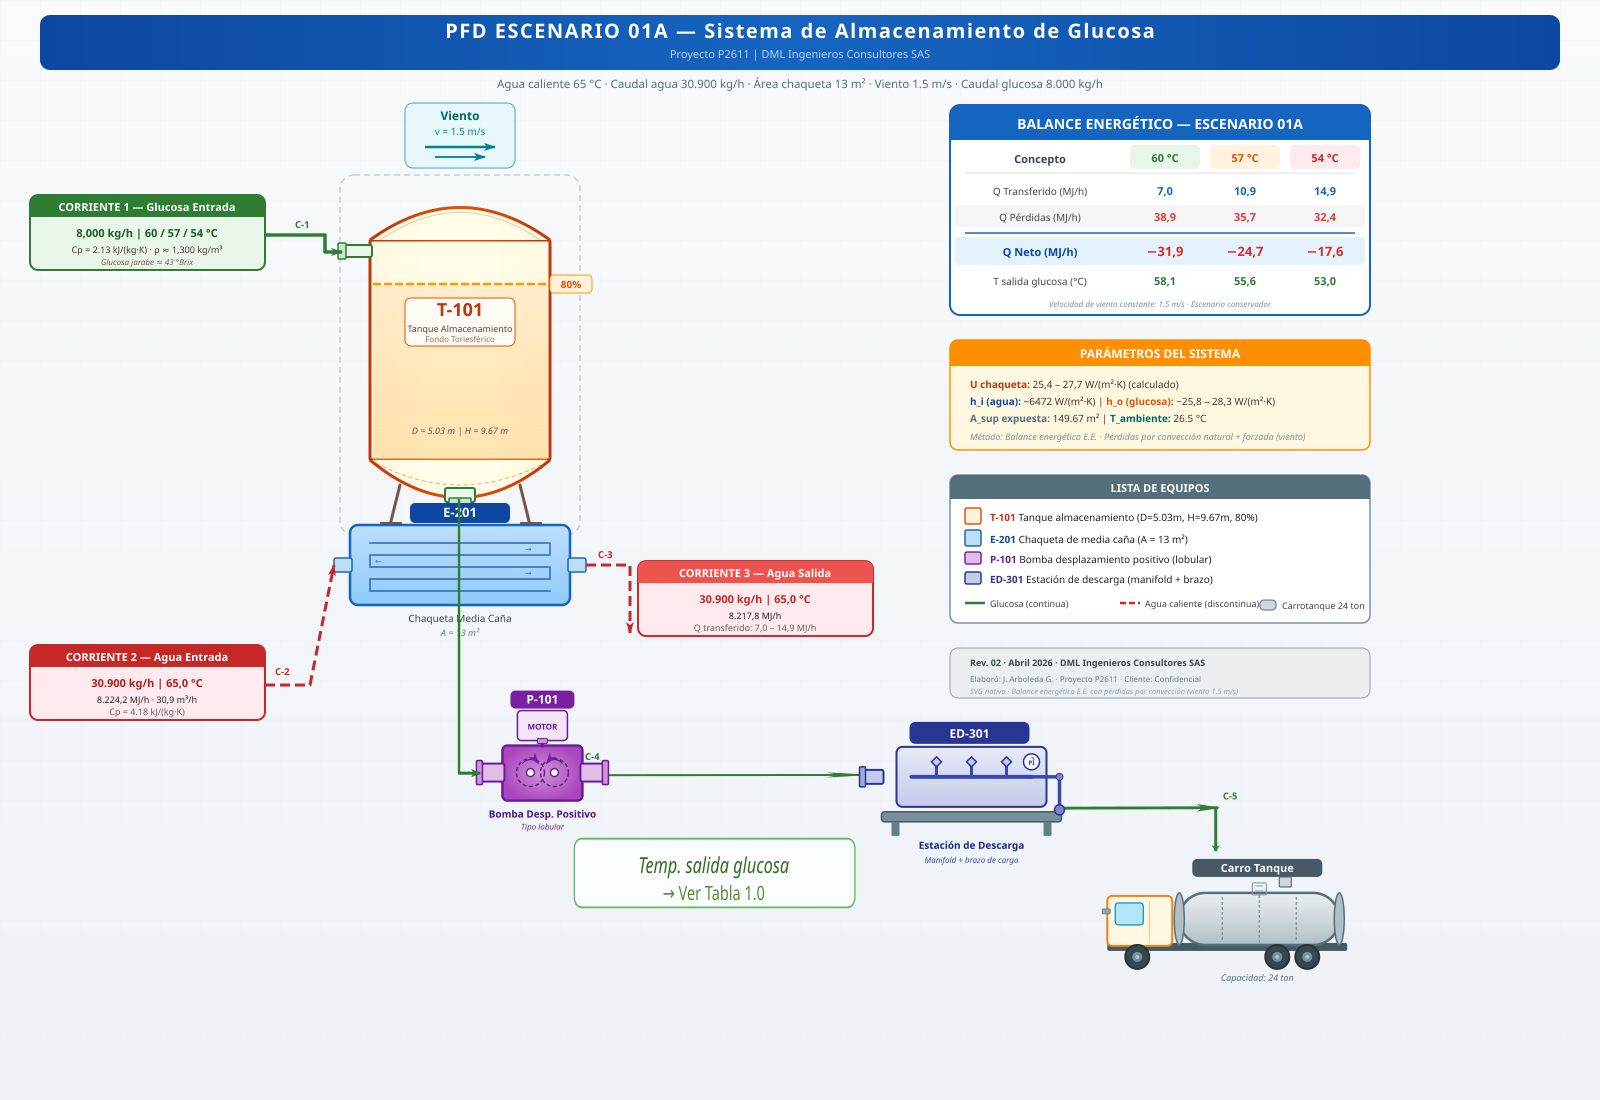
\includegraphics[width=\textwidth]{../../results/PFD_Escenario_01A.pdf}
\caption{Diagrama de flujo de proceso (PFD) --- Escenario 01A: agua de servicio a 65$^\circ$C, caudal 30,900~kg/h, \'{a}rea de transferencia 13~m$^2$, velocidad de viento 1.5~m/s. Se comparan tres temperaturas de entrada de glucosa.}
\label{fig:pfd_escenario_01a}
\end{figure}



El Escenario 01A muestra que, con las condiciones base del dise\~{n}o, el sistema presenta un balance energ\'{e}tico neto negativo en todas las condiciones evaluadas. Las p\'{e}rdidas t\'{e}rmicas exceden el calor transferido desde la chaqueta, y la glucosa sale del tanque a temperatura inferior a la de entrada.


\section{Escenario 01B}

En este escenario se aumenta el flujo de agua de calentamiento para alcanzar una velocidad de 2.5~m/s en el ducto de calentamiento (chaqueta) ($v_s=2.5$~m/s), manteniendo la temperatura del agua a 65$^\circ$C y el \'{a}rea de transferencia en 13~m$^2$. Se eval\'{u}an las mismas tres temperaturas de entrada de glucosa.

\begin{figure}[H]
\centering
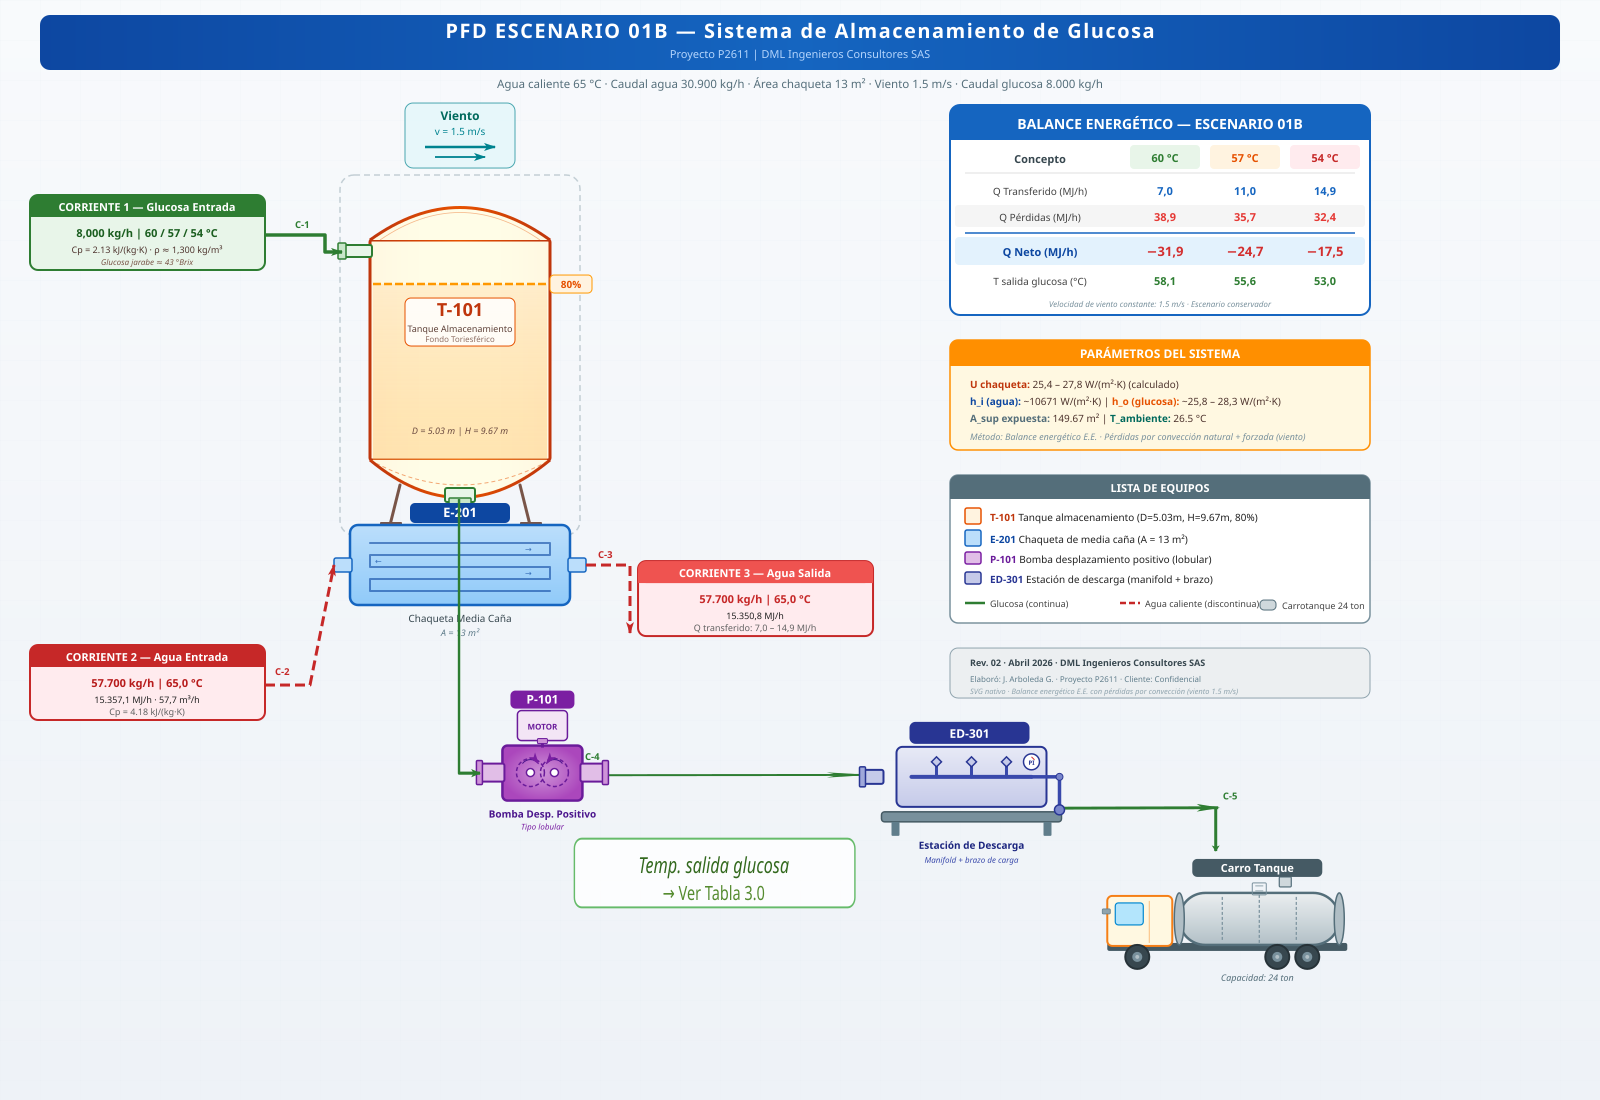
\includegraphics[width=\textwidth]{../../results/PFD_Escenario_01B.pdf}
\caption{Diagrama de flujo de proceso (PFD) --- Escenario 01B: agua de servicio a 65$^\circ$C, caudal 57,700~kg/h ($v=2.5$~m/s), \'{a}rea de transferencia 13~m$^2$, velocidad de viento 1.5~m/s.}
\label{fig:pfd_escenario_01b}
\end{figure}

\begin{table}[H]
\centering
\footnotesize
\caption{Comparativa de temperaturas de salida --- Escenarios 01B-1, 01B-2 y 01B-3 (Velocidad viento 1.5~m/s).}
\label{tab:comparativa_01b}
\begin{tabularx}{\textwidth}{@{}Xcc@{}}
\toprule
\textbf{Escenario} & \textbf{$T_{\text{glucosa, entrada}}$ [$^\circ$C]} & \textbf{$T_{\text{glucosa, salida}}$ [$^\circ$C]} \\
\midrule
01B-1 & 60.0 & 58.2 \\
01B-2 & 57.0 & 55.7 \\
01B-3 & 54.0 & 53.1 \\
\bottomrule
\end{tabularx}
\end{table}

El aumento de velocidad del agua de 1.34~m/s a 2.5~m/s no produce una mejora t\'{e}rmica apreciable. Los resultados son pr\'{a}cticamente id\'{e}nticos a los del Escenario 01A, confirmando que la resistencia t\'{e}rmica dominante se encuentra del lado de la glucosa.


\section{Escenario 01C}

En este escenario se eleva la temperatura del agua de calentamiento a 75$^\circ$C, manteniendo la velocidad aumentada de 2.5~m/s y el \'{a}rea de 13~m$^2$. El objetivo es determinar si el incremento de 10$^\circ$C en la temperatura del fluido calefactor permite alcanzar temperaturas de salida de glucosa $\geq$57$^\circ$C.

\begin{figure}[H]
\centering
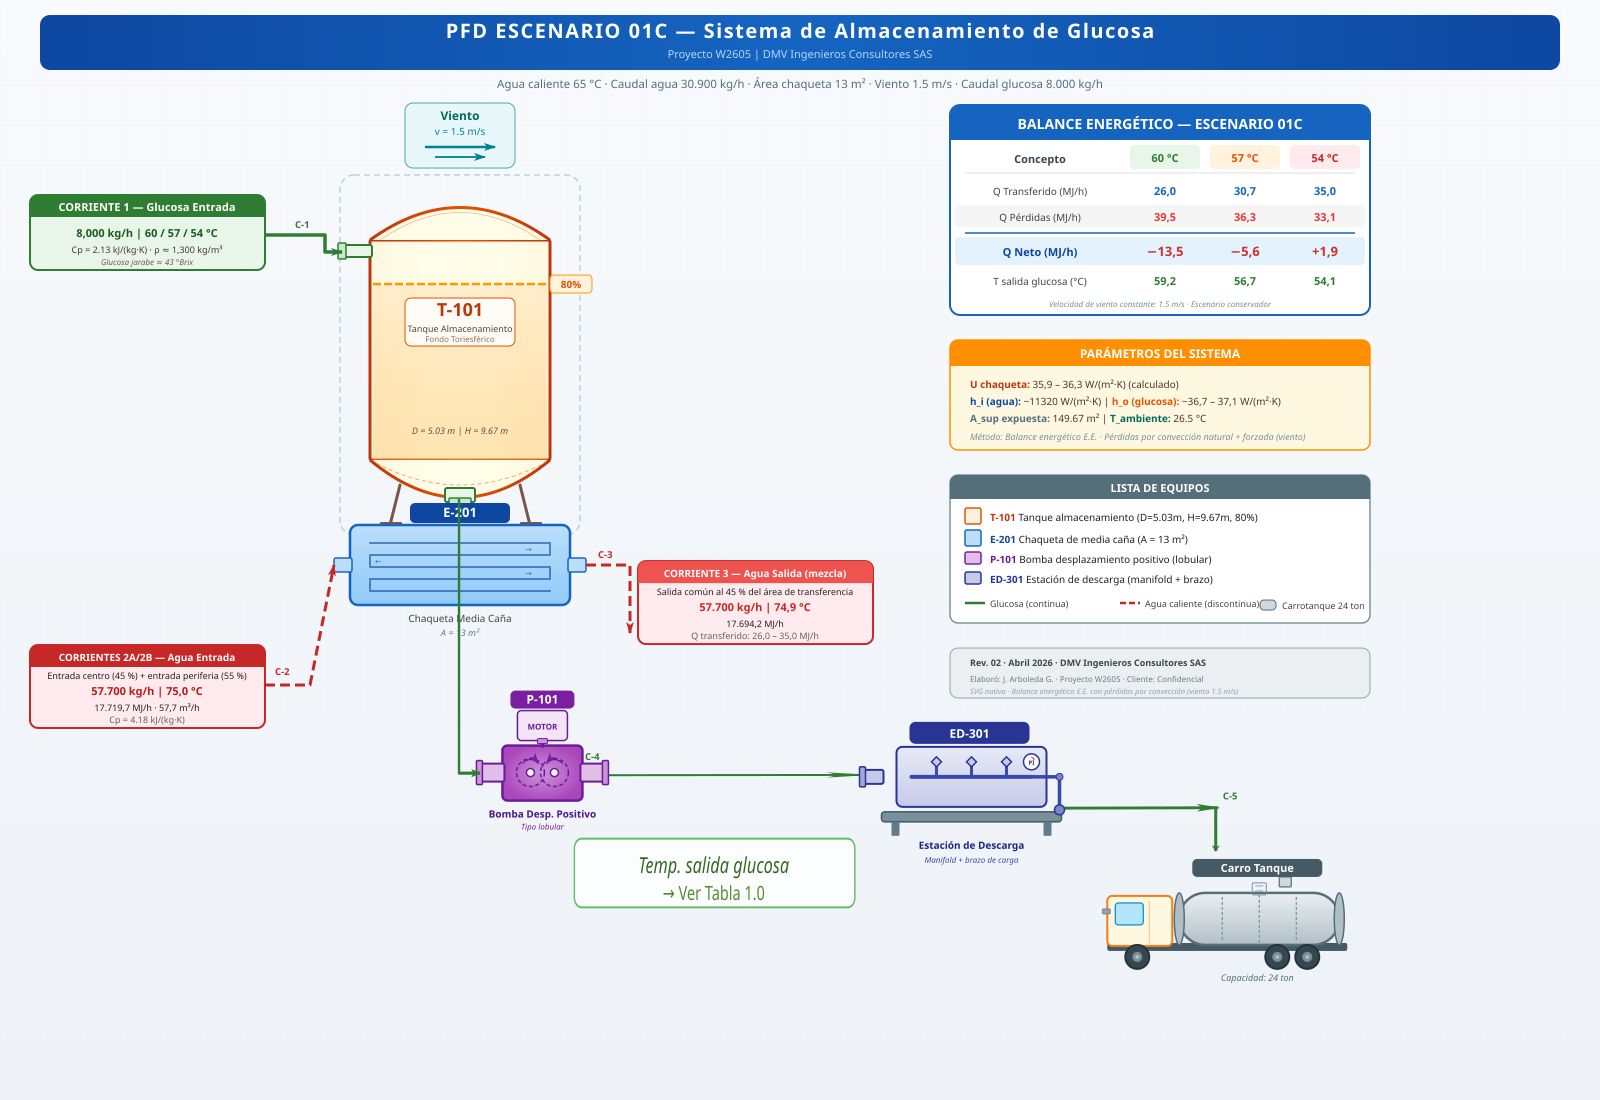
\includegraphics[width=\textwidth]{../../results/PFD_Escenario_01C.pdf}
\caption{Diagrama de flujo de proceso (PFD) --- Escenario 01C: agua de servicio a 75$^\circ$C, caudal 57,700~kg/h ($v=2.5$~m/s), \'{a}rea de transferencia 13~m$^2$, velocidad de viento 1.5~m/s.}
\label{fig:pfd_escenario_01c}
\end{figure}

\begin{table}[H]
\centering
\footnotesize
\caption{Comparativa de temperaturas de salida --- Escenarios 01C-1, 01C-2 y 01C-3 (Velocidad viento 1.5~m/s).}
\label{tab:comparativa_01c}
\begin{tabularx}{\textwidth}{@{}Xcc@{}}
\toprule
\textbf{Escenario} & \textbf{$T_{\text{glucosa, entrada}}$ [$^\circ$C]} & \textbf{$T_{\text{glucosa, salida}}$ [$^\circ$C]} \\
\midrule
01C-1 & 60.0 & 59.2 \\
01C-2 & 57.0 & 56.7 \\
01C-3 & 54.0 & 54.1 \\
\bottomrule
\end{tabularx}
\end{table}

El incremento de la temperatura del agua a 75$^\circ$C mejora significativamente el desempe\~{n}o t\'{e}rmico. Para el caso con entrada de glucosa a 54$^\circ$C (01C-3), el balance neto es ligeramente positivo (+1.9~MJ/h), aunque la temperatura de salida (54.1$^\circ$C) permanece por debajo del l\'{i}mite operativo de 57$^\circ$C.


\section{Escenario 02A}

Este escenario eval\'{u}a el impacto de duplicar el \'{a}rea de transferencia de la chaqueta a 28~m$^2$, manteniendo el agua a 75$^\circ$C, el caudal de 57,700~kg/h ($v=2.5$~m/s) y la velocidad de viento de 1.5~m/s. Se analizan las tres temperaturas de entrada de glucosa.

\begin{figure}[H]
\centering
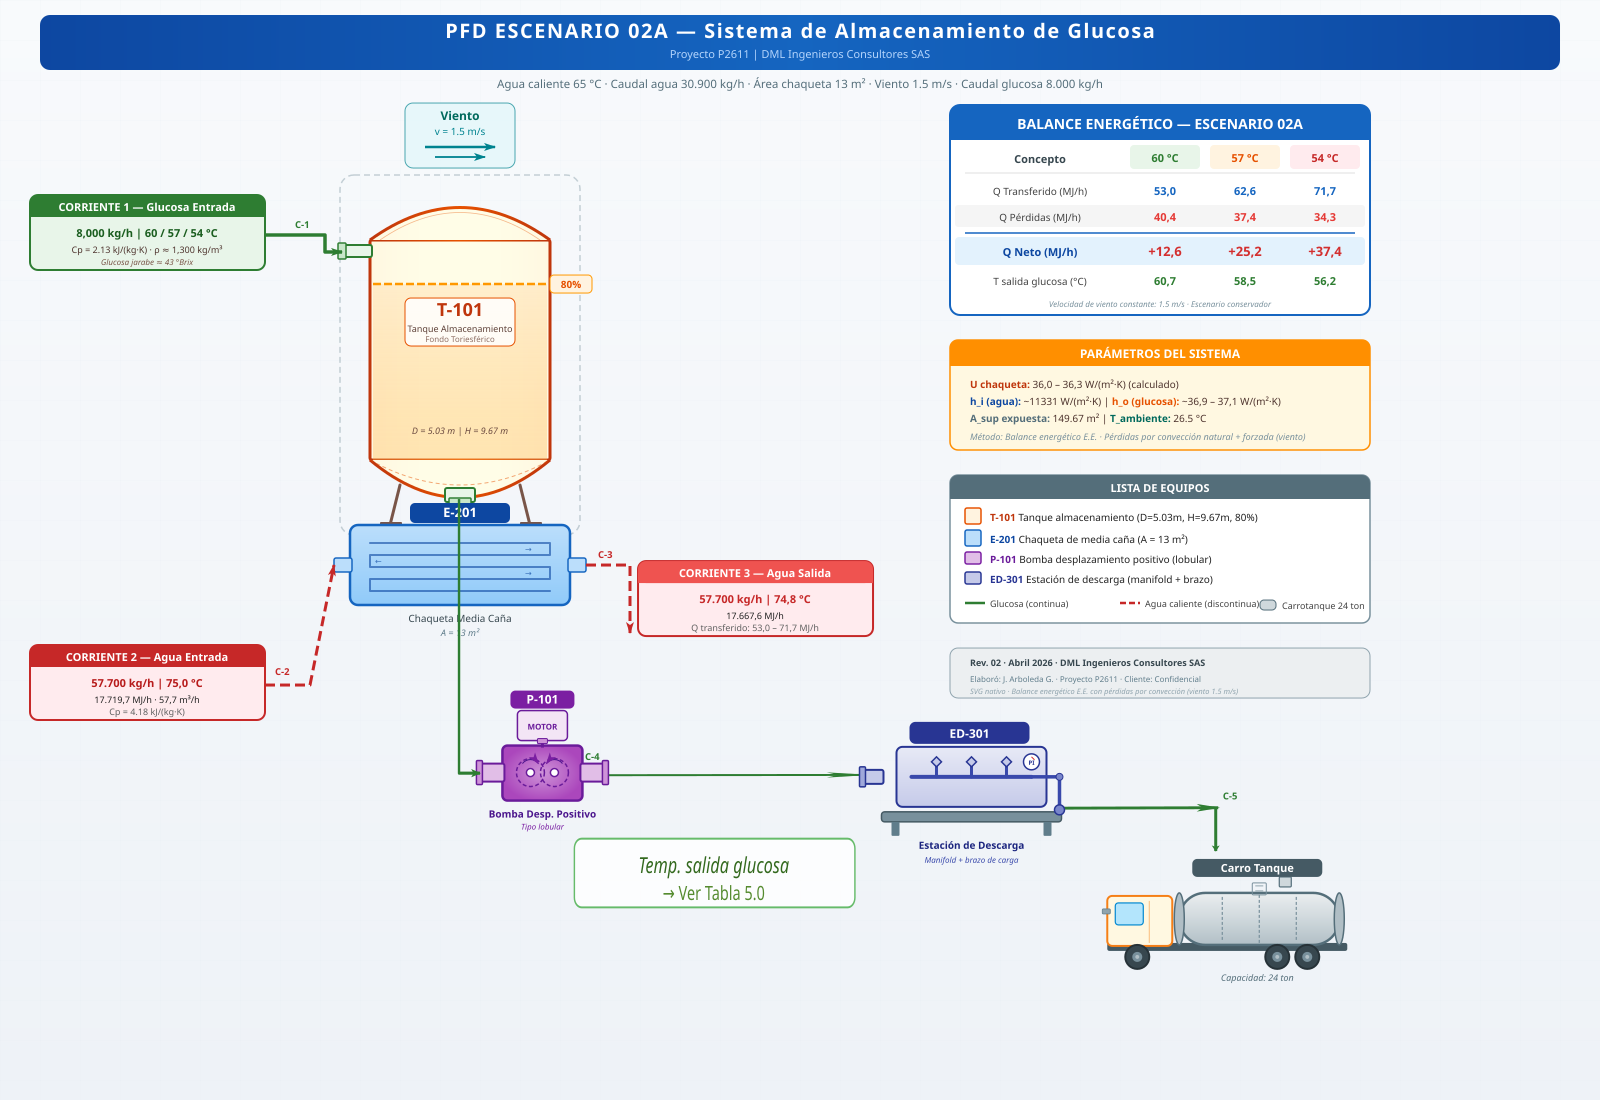
\includegraphics[width=\textwidth]{../../results/PFD_Escenario_02A.pdf}
\caption{Diagrama de flujo de proceso (PFD) --- Escenario 02A: agua de servicio a 75$^\circ$C, caudal 57,700~kg/h ($v=2.5$~m/s), \'{a}rea de transferencia 28~m$^2$, velocidad de viento 1.5~m/s.}
\label{fig:pfd_escenario_02a}
\end{figure}

\begin{table}[H]
\centering
\footnotesize
\caption{Comparativa de temperaturas de salida --- Escenarios 02A-1, 02A-2 y 02A-3 (Velocidad viento 1.5~m/s).}
\label{tab:comparativa_02a}
\begin{tabularx}{\textwidth}{@{}Xcc@{}}
\toprule
\textbf{Escenario} & \textbf{$T_{\text{glucosa, entrada}}$ [$^\circ$C]} & \textbf{$T_{\text{glucosa, salida}}$ [$^\circ$C]} \\
\midrule
02A-1 & 60.0 & 60.7 \\
02A-2 & 57.0 & 58.5 \\
02A-3 & 54.0 & 56.2 \\
\bottomrule
\end{tabularx}
\end{table}

Al aumentar el \'{a}rea de transferencia a 28~m$^2$, el balance energ\'{e}tico neto se vuelve positivo en todos los casos. Incluso con glucosa entrando a 54$^\circ$C, la temperatura de salida alcanza 56.2$^\circ$C, acerc\'{a}ndose al l\'{i}mite operativo requerido de 57$^\circ$C. Este resultado destaca la importancia cr\'{i}tica del \'{a}rea de transferencia en el dise\~{n}o de la chaqueta.


\section{Resumen Resultados}

La Tabla~\ref{tab:resultados_globales} consolida los resultados de temperatura de salida de glucosa para los doce subescenarios evaluados, a una velocidad de viento representativa de 1.5~m/s. Las celdas de temperatura se resaltan en \colorbox{green!25}{verde} cuando se cumple la condici\'{o}n operativa m\'{i}nima ($T_{\text{sal}} \geq 57^\circ$C) y en \colorbox{red!20}{rojo} cuando no se cumple. 

\begin{table}[H]
\centering
\footnotesize
\caption{Consolidado de resultados --- Temperatura de salida de glucosa y balance energ\'{e}tico por subescenario a $v_{\text{viento}}=1.5$~m/s.
Celdas en \protect\colorbox{green!25}{verde}: operaci\'{o}n viable ($T_{\text{sal}}\geq57^\circ$C);
en \protect\colorbox{red!20}{rojo}: operaci\'{o}n no viable.}
\label{tab:resultados_globales}
\begin{tabularx}{\textwidth}{@{}Xccccr@{}}
\toprule
\textbf{Escenario} &
\textbf{$T_{\text{agua}}$} &
\textbf{$v_{\text{agua}}$} &
\textbf{$T_{\text{gluc,in}}$} &
\textbf{$T_{\text{gluc,sal}}$ ($^\circ$C)} &
\textbf{Bal. neto} \\
 & ($^\circ$C) & (m/s) & ($^\circ$C) & $v_{\text{viento}}=1.5$~m/s & (MJ/h) \\
\midrule
\multicolumn{6}{@{}l}{\textit{Escenario 01A --- Agua 65$^\circ$C, caudal 30\,900~kg/h, $A=13$~m$^2$}} \\[2pt]
01A-1 & 65 & 1.34 & 60 & \cellcolor{green!25}\textbf{58.1} & $-$31.9 \\
01A-2 & 65 & 1.34 & 57 & \cellcolor{red!20}\textbf{55.6} & $-$24.7 \\
01A-3 & 65 & 1.34 & 54 & \cellcolor{red!20}\textbf{53.0} & $-$17.6 \\
\midrule
\multicolumn{6}{@{}l}{\textit{Escenario 01B --- Agua 65$^\circ$C, caudal 57\,700~kg/h, $A=13$~m$^2$}} \\[2pt]
01B-1 & 65 & 2.50 & 60 & \cellcolor{green!25}\textbf{58.1} & $-$31.9 \\
01B-2 & 65 & 2.50 & 57 & \cellcolor{red!20}\textbf{55.6} & $-$24.7 \\
01B-3 & 65 & 2.50 & 54 & \cellcolor{red!20}\textbf{53.0} & $-$17.5 \\
\midrule
\multicolumn{6}{@{}l}{\textit{Escenario 01C --- Agua 75$^\circ$C, caudal 57\,700~kg/h, $A=13$~m$^2$}} \\[2pt]
01C-1 & 75 & 2.50 & 60 & \cellcolor{green!25}\textbf{59.2} & $-$13.5 \\
01C-2 & 75 & 2.50 & 57 & \cellcolor{red!20}\textbf{56.7} & $-$5.6 \\
01C-3 & 75 & 2.50 & 54 & \cellcolor{red!20}\textbf{54.1} & $+$1.9 \\
\midrule
\multicolumn{6}{@{}l}{\textit{Escenario 02A --- Agua 75$^\circ$C, caudal 57\,700~kg/h, $A=28$~m$^2$}} \\[2pt]
02A-1 & 75 & 2.50 & 60 & \cellcolor{green!25}\textbf{60.7} & $+$12.6 \\
02A-2 & 75 & 2.50 & 57 & \cellcolor{green!25}\textbf{58.5} & $+$25.2 \\
02A-3 & 75 & 2.50 & 54 & \cellcolor{red!20}\textbf{56.2} & $+$37.4 \\
\bottomrule
\end{tabularx}
\end{table}

Los resultados muestran que los Escenarios 01A y 01B presentan comportamientos t\'{e}rmicos pr\'{a}cticamente id\'{e}nticos a $v_{\text{viento}}=1.5$~m/s, confirmando que el incremento de velocidad del agua no compensa las p\'{e}rdidas t\'{e}rmicas cuando la resistencia dominante est\'{a} del lado de la glucosa. El Escenario 01C mejora las temperaturas de salida gracias al aumento de 10$^\circ$C en la temperatura del agua, pero a\'{u}n as\'{i} no logra mantener la glucosa por encima de 57$^\circ$C para las entradas m\'{a}s bajas. El \'{u}nico escenario que garantiza operaci\'{o}n viable  para todas las temperaturas de entrada evaluadas es el 02A-1 y 02A-2


\section{Observaciones y recomendaciones: revisi\'{o}n t\'{e}rmica}


1) Con el diseño entregado, la salida de la glucosa se mantendrá por encima de los 57$^\circ$C solo si la temperatura a la entrada al tanque de la glucosa está por encima de 59.5$^\circ$C; por debajo de esta temperatura no se tendrá la condición óptima de salida de la glucosa, siendo muy crítico el caso en que se suministre al tanque glucosa a 54$^\circ$C, ya que la salida de la glucosa estaría alrededor de los 53$^\circ$C.

2) Como puede verse de la tabla resumen para garantizar una temperatura de salida por encima de la temperatura minima se debe cumplir con la condicion del escenario 4, inclusive recomendamos aumentar el area a 30 m2

3) Para disminuir las perdidas por conveccion en el tanque se recomienda mejorar el aislamiento.



\section{Revisi\'{o}n estructural}

El an\'{a}lisis estructural del tanque Tag 53A-90A-0056 se desarroll\'{o} mediante el m\'{e}todo de elementos finitos (FEA) en el software ANSYS Mechanical 2025 (NUBE). La geometr\'{i}a tridimensional se construy\'{o} a partir de los planos mec\'{a}nicos suministrados por Ingredion S.A. (\texttt{REV0DMI17160102}, feb.~2026), incorporando el cuerpo cil\'{i}ndrico, el fondo torisf\'{e}rico de reemplazo, la chaqueta de media ca\~{n}a tipo perfil rectangular y los anclajes de base. Se evaluaron las condiciones de carga combinada m\'{a}s representativas para el dise\~{n}o: presi\'{o}n hidrost\'{a}tica a su nivel m\'{a}ximo de operaci\'{o}n normal (222.8~m\textsuperscript{3} / 314~t) y gradiente t\'{e}rmico de calentamiento a 75\,$^\circ$C en el fondo, frente a un cuerpo cil\'{i}ndrico a temperatura ambiente.

\begin{figure}[H]
\centering
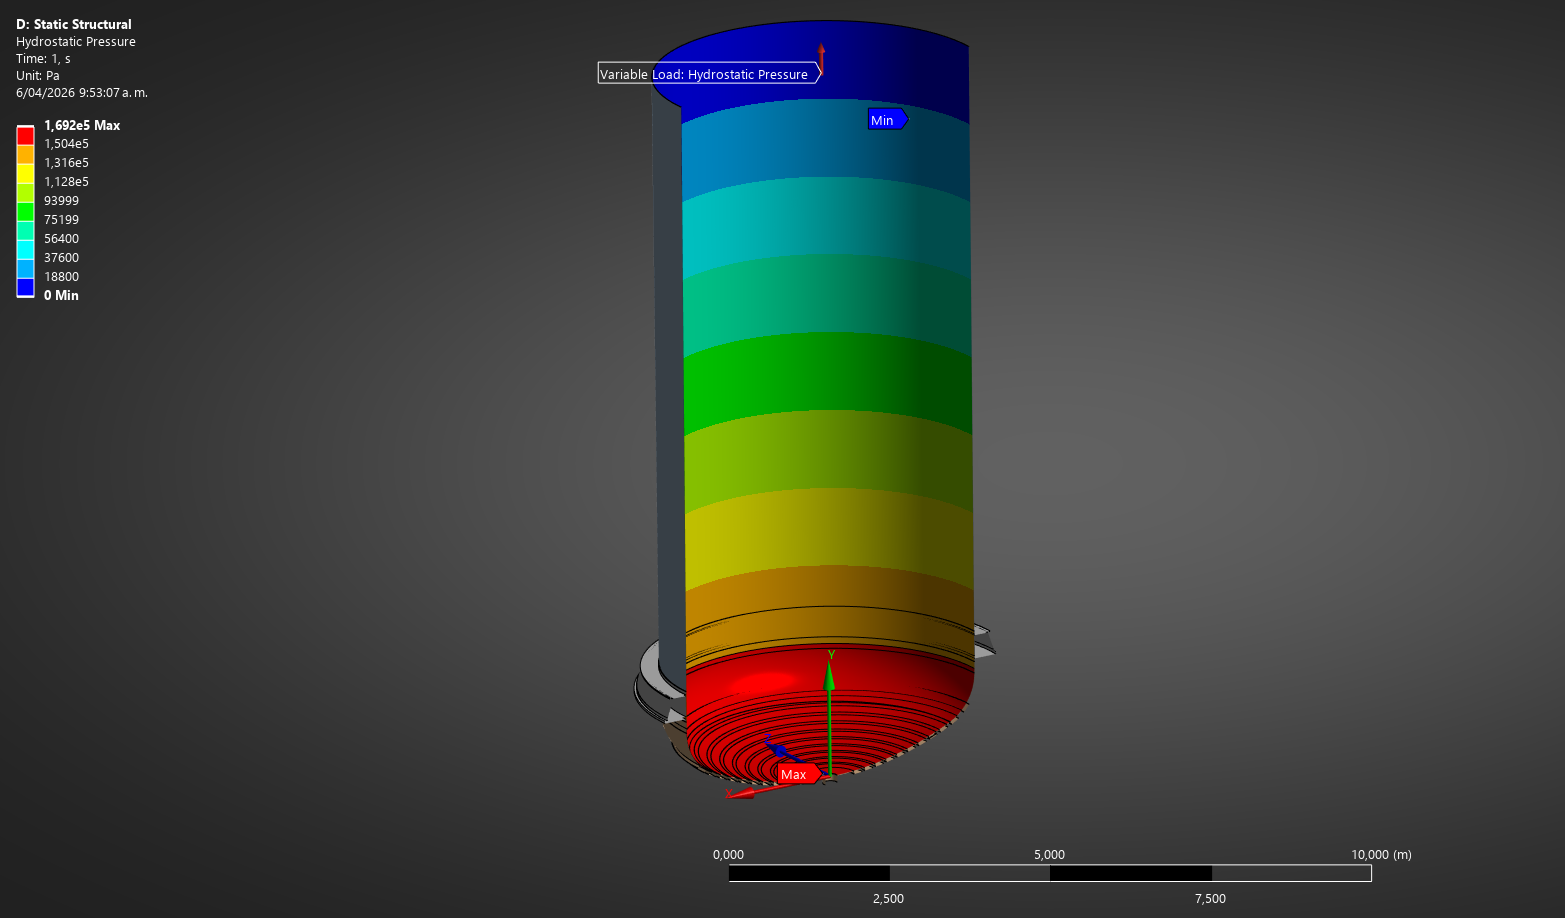
\includegraphics[width=0.65\textwidth]{../../results/figures/fea1.png}
\caption{Distribuci\'{o}n de presi\'{o}n hidrost\'{a}tica sobre la geometr\'{i}a del tanque. La presi\'{o}n m\'{a}xima ($\sim$1.69$\times$10$^5$~Pa) se concentra en la zona inferior del fondo torisf\'{e}rico, decreciendo progresivamente hacia la parte superior del cilindro.}
\label{fig:fea1}
\end{figure}

La Figura~\ref{fig:fea1} ilustra la distribuci\'{o}n de presi\'{o}n hidrost\'{a}tica ejercida por la columna de glucosa. El valor m\'{a}ximo ($\sim$0.17~MPa) se localiza en el v\'{e}rtice del fondo torisf\'{e}rico, conforme al perfil de carga hidrost\'{a}tica $p = \rho g h$. Este resultado es consistente con la teor\'{i}a de recipientes a presi\'{o}n y constituye la carga mec\'{a}nica dominante para el dimensionamiento del fondo de reemplazo.

\begin{figure}[H]
\centering
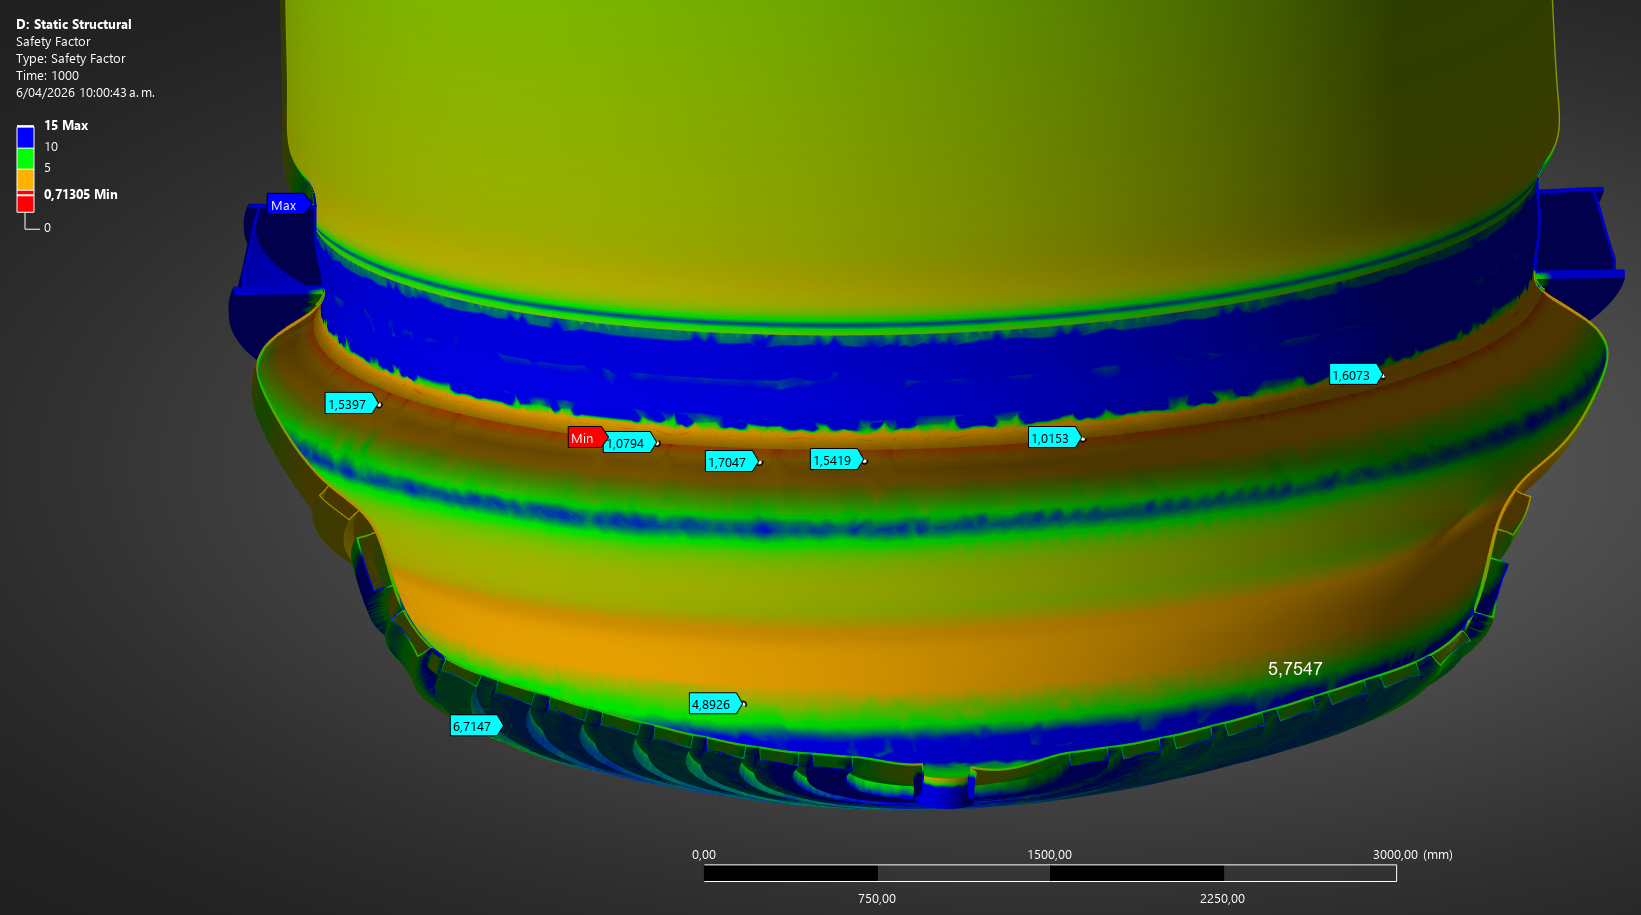
\includegraphics[width=0.85\textwidth]{../../results/figures/fea3.png}
\caption{Mapa de factor de seguridad (safety factor) obtenido por FEA bajo carga combinada hidrost\'{a}tica y t\'{e}rmica (75\,$^\circ$C). El valor m\'{i}nimo global ($\sim$0.71) se registra en la uni\'{o}n fondo-cilindro. Los anclajes de la chaqueta presentan factores de seguridad entre 1.0 y 1.7, mientras que el fondo propiamente dicho exhibe m\'{a}rgenes de 4.9 a 6.7 y el cilindro superiores a 15.}
\label{fig:fea3}
\end{figure}

La Figura~\ref{fig:fea3} presenta el mapa de factor de seguridad, donde se identifican tres zonas de inter\'{e}s estructural. La zona m\'{a}s cr\'{i}tica es la uni\'{o}n fondo-cilindro, con un factor de seguridad m\'{i}nimo de aproximadamente 0.71, lo que indica un sobreesfuerzo local a su nivel m\'{a}ximo de operaci\'{o}n normal (222.8~m\textsuperscript{3} / 314~t). Esta concentraci\'{o}n de esfuerzos es propia de la discontinuidad geom\'{e}trica en fondos torisf\'{e}ricos y se ve acentuada por el gradiente t\'{e}rmico diferencial. Los puntos de anclaje de la chaqueta de media ca\~{n}a constituyen un segundo foco de atenci\'{o}n, con factores de seguridad entre 1.0 y 1.7, atribuibles a las discontinuidades geom\'{e}tricas introducidas por las soldaduras de filete. En contraste, el fondo torisf\'{e}rico promedio presenta m\'{a}rgenes de 4.9 a 6.7, y el cuerpo cil\'{i}ndrico opera con factores superiores a 15, evidenciando que la virola no es el elemento restrictivo.

\subsection{Observaciones y recomendaciones}

\subsubsection{Observaciones}

1) Cuando el tanque se llena a su nivel m\'{a}ximo de operaci\'{o}n normal (222.8~m\textsuperscript{3} / 314~t), el factor de seguridad en la uni\'{o}n fondo-cilindro desciende por debajo de la unidad ($FS \approx 0.71$), lo que evidencia una condici\'{o}n de sobreesfuerzo local. En consecuencia, el an\'{a}lisis FEA establece que el l\'{i}mite operativo seguro para garantizar un factor de seguridad m\'{i}nimo de 1.3 es 178.2~m\textsuperscript{3} (251~t).

2) Bajo el escenario de corrosi\'{o}n-fatiga (tasa de degradaci\'{o}n 0.120~mm/a\~{n}o, determinada en el estudio de espesores \textit{Informe Tanque Almacenamiento de Glucosa No.~4 --- Anillo\_V1} y \textit{MT-ME-003 Tanque 5 Espesores}, asociada a la nueva condici\'{o}n de 75\,$^\circ$C y ciclicidad t\'{e}rmica), la vida \'{u}til proyectada del fondo nuevo hasta alcanzar el l\'{i}mite de retiro del 10\% (8.1~mm) es de aproximadamente 7.5 a\~{n}os. En el escenario hist\'{o}rico menos agresivo (0.0625~mm/a\~{n}o), la vida \'{u}til se extiende a $\sim$14.4 a\~{n}os.

\subsubsection{Recomendaciones}

1) Los anclajes de la chaqueta de media ca\~{n}a y la zona de la uni\'{o}n fondo-cilindro deben incluirse de manera expl\'{i}cita en el programa de inspecci\'{o}n por Ensayos No Destructivos (END), preferiblemente mediante t\'{e}cnicas de PAUT o UT, con una periodicidad bianual que permita la detecci\'{o}n temprana de fisuraci\'{o}n por fatiga t\'{e}rmica.

2) Establecer un programa de monitoreo de espesores que valide la tasa real de degradaci\'{o}n durante los primeros tres a\~{n}os de operaci\'{o}n.

3) Desarrollar un estudio de refuerzo estructural focalizado en la uni\'{o}n fondo-cilindro, con el objetivo de mejorar el factor de seguridad actual ($FS \approx 0.71$ a nivel m\'{a}ximo de operaci\'{o}n) y garantizar m\'{a}rgenes normativos compatibles con ASME~VIII Div.~1. Este estudio debe evaluar alternativas t\'{e}cnicas tales como el incremento localizado del espesor, la instalaci\'{o}n de anillos de rigidizaci\'{o}n perimetrales o la aplicaci\'{o}n de placas de refuerzo (pads), validando la efectividad de cada opci\'{o}n mediante un modelo actualizado de elementos finitos (FEA).

\end{document}
